\begin{figure}[!p]
\centering
\resizebox{\linewidth}{!}{\sffamily
{(a)} \begin{tabular}{c|c|c|c|c|c|c|c}
\texttt{\#99} (364 nt) & Boltzmann prob. & ensemble defect & struct. distance & energy gap & & & \\
``Shooting Star'' & $p(\vecystar \mid \vecx)$$(\uparrow)$ & \NED$(\vecx, \vecystar)$$(\downarrow)$ & $d(\MFE(\vecx), \vecystar)$$(\downarrow)$ & \DDG$(\vecx, \vecystar)$$(\downarrow)$ & is \MFE & is uMFE & designable \\
\hline
EliteDesign ($N=500$) & {\boldmath$6.16 \times 10^{-7}$} & \textbf{0.107} & \textbf{20} & \textbf{3.8 kcal/mol} & No & No & \multirow{2}{*}{No} \\
SamplingDesign & $5.50 \times 10^{-10}$ & 0.173 & \textbf{20} & 7.8 kcal/mol & No & No & \\
\hline
Probability ceiling & $5.15 \times 10^{-4}$ & --- & --- & --- & --- & --- & --- \\
\end{tabular}}\\[5pt]
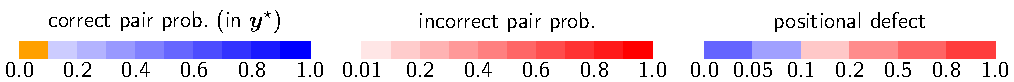
\includegraphics[width=0.9\linewidth]{figures/structures/legend}\\[3pt]
{\sffamily\small
\begin{tabular}{@{}c@{\hspace{0.01\linewidth}}c@{\hspace{0.01\linewidth}}c@{}}
(b) Target \vecystar & (c) \MFE structure of EliteDesign ($N=500$) & (d) \MFE structure of SamplingDesign \\[2pt]
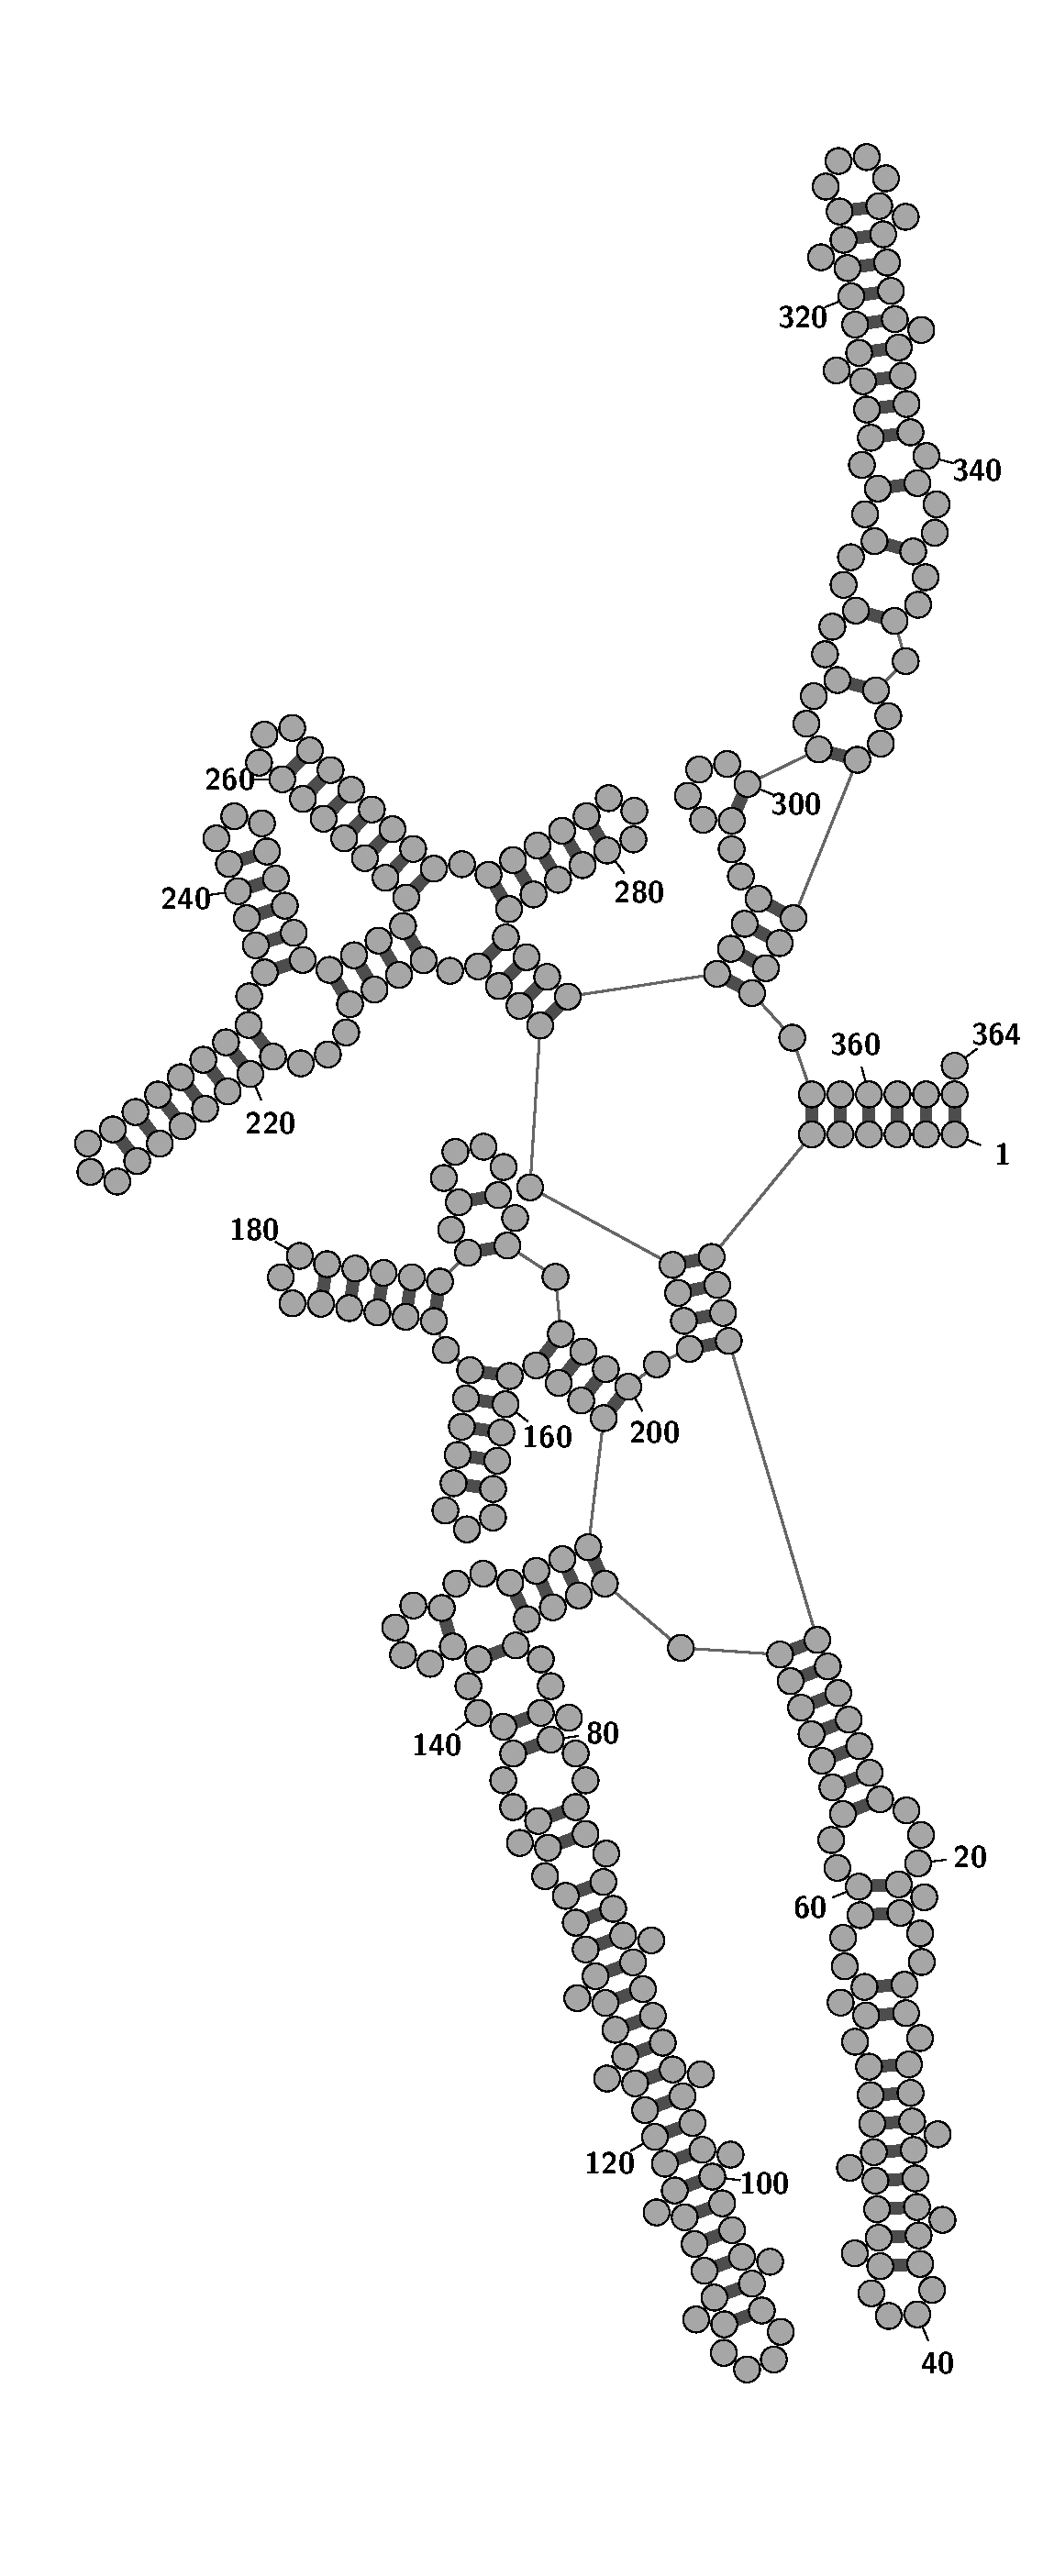
\includegraphics[height=4.85in]{figures/structures/target_99} &
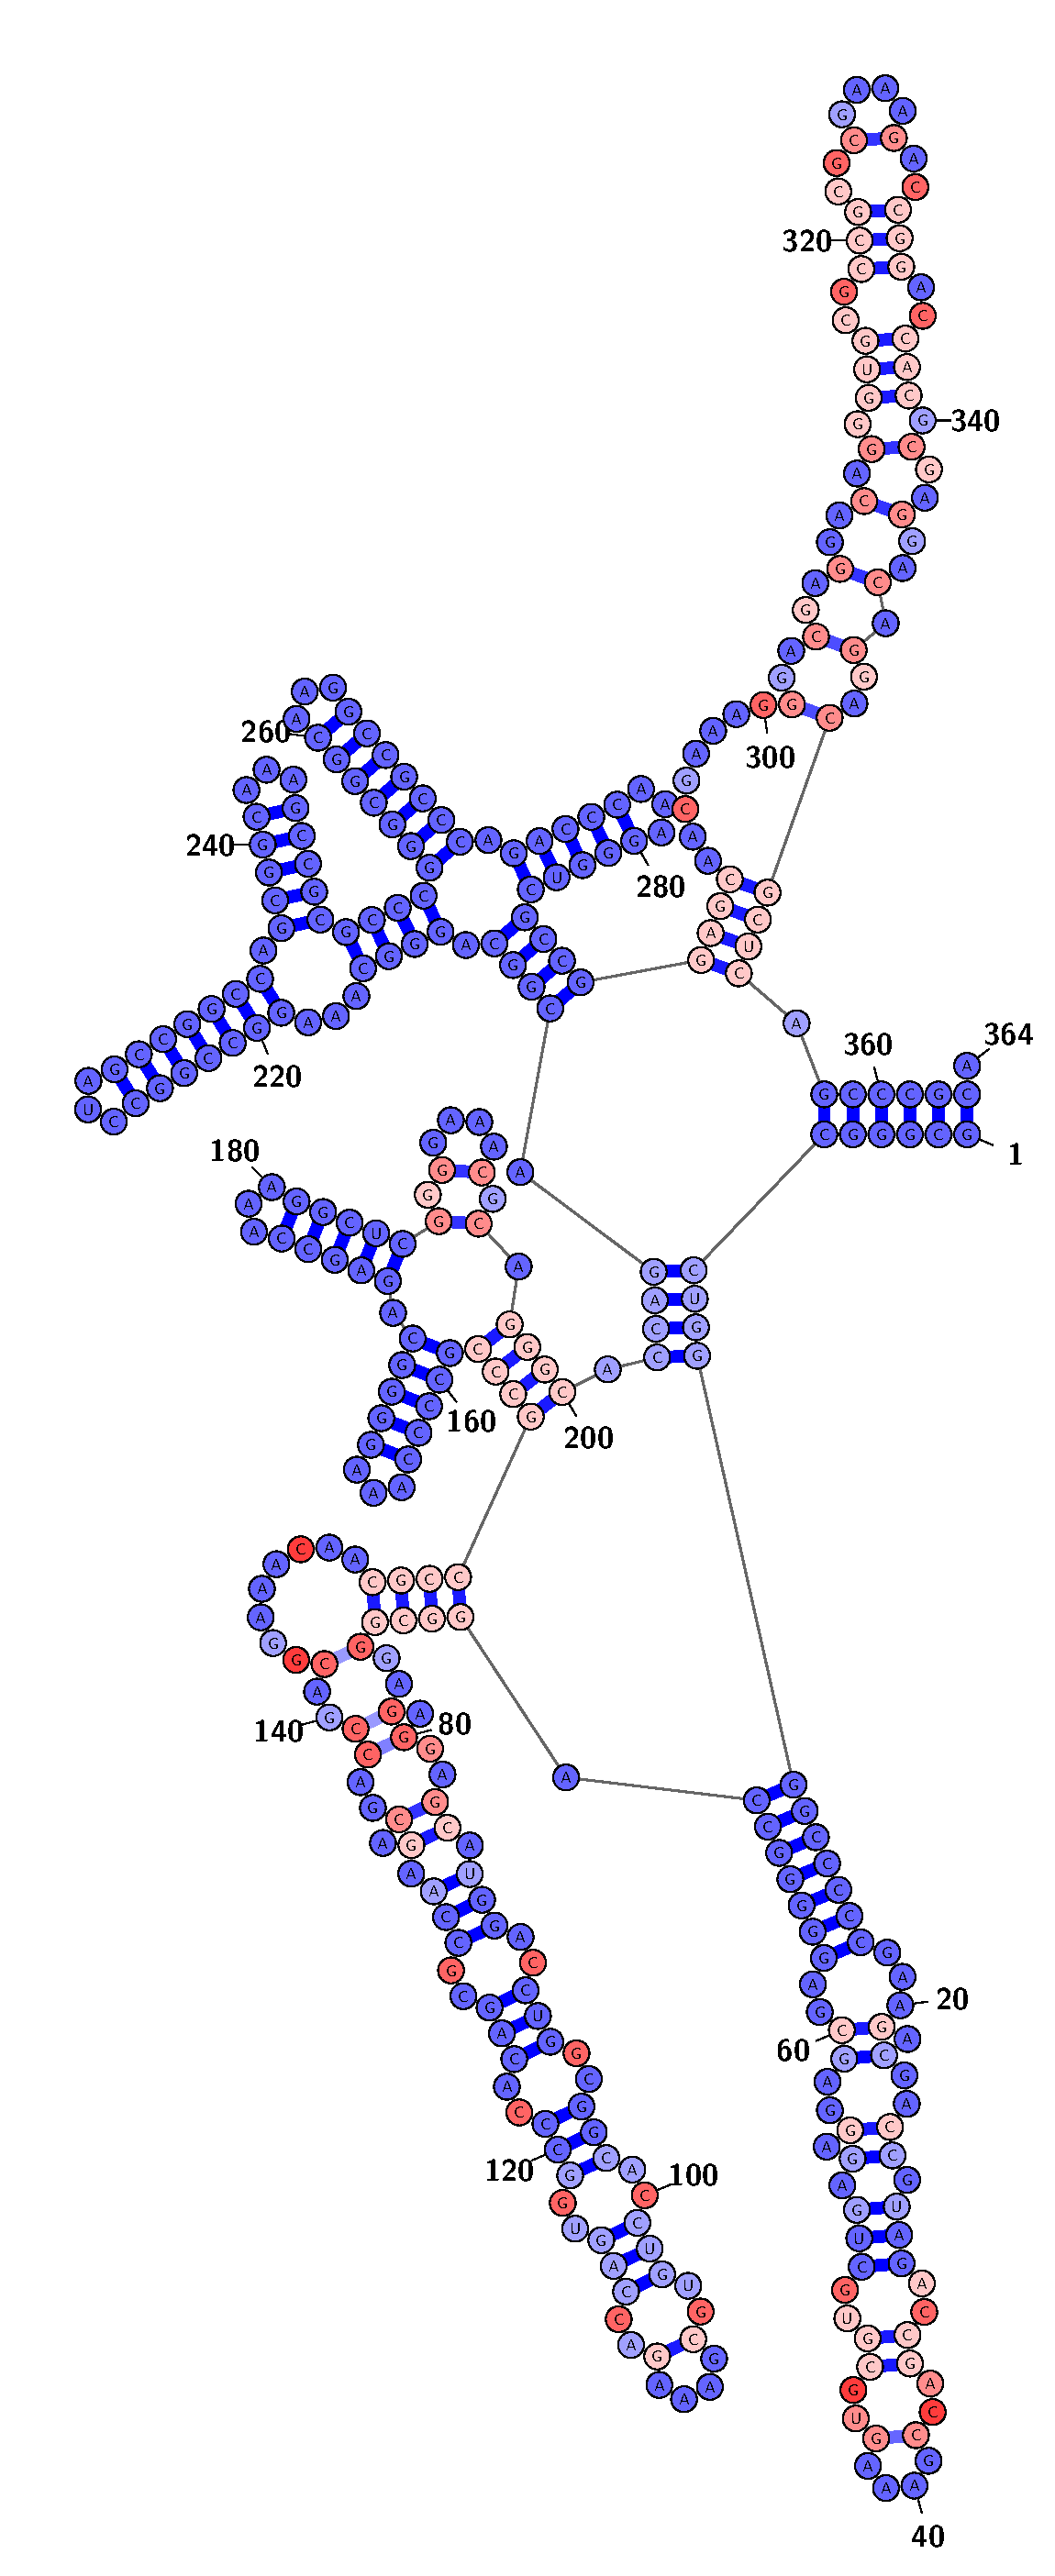
\includegraphics[height=4.85in]{figures/structures/structure_99_elite} &
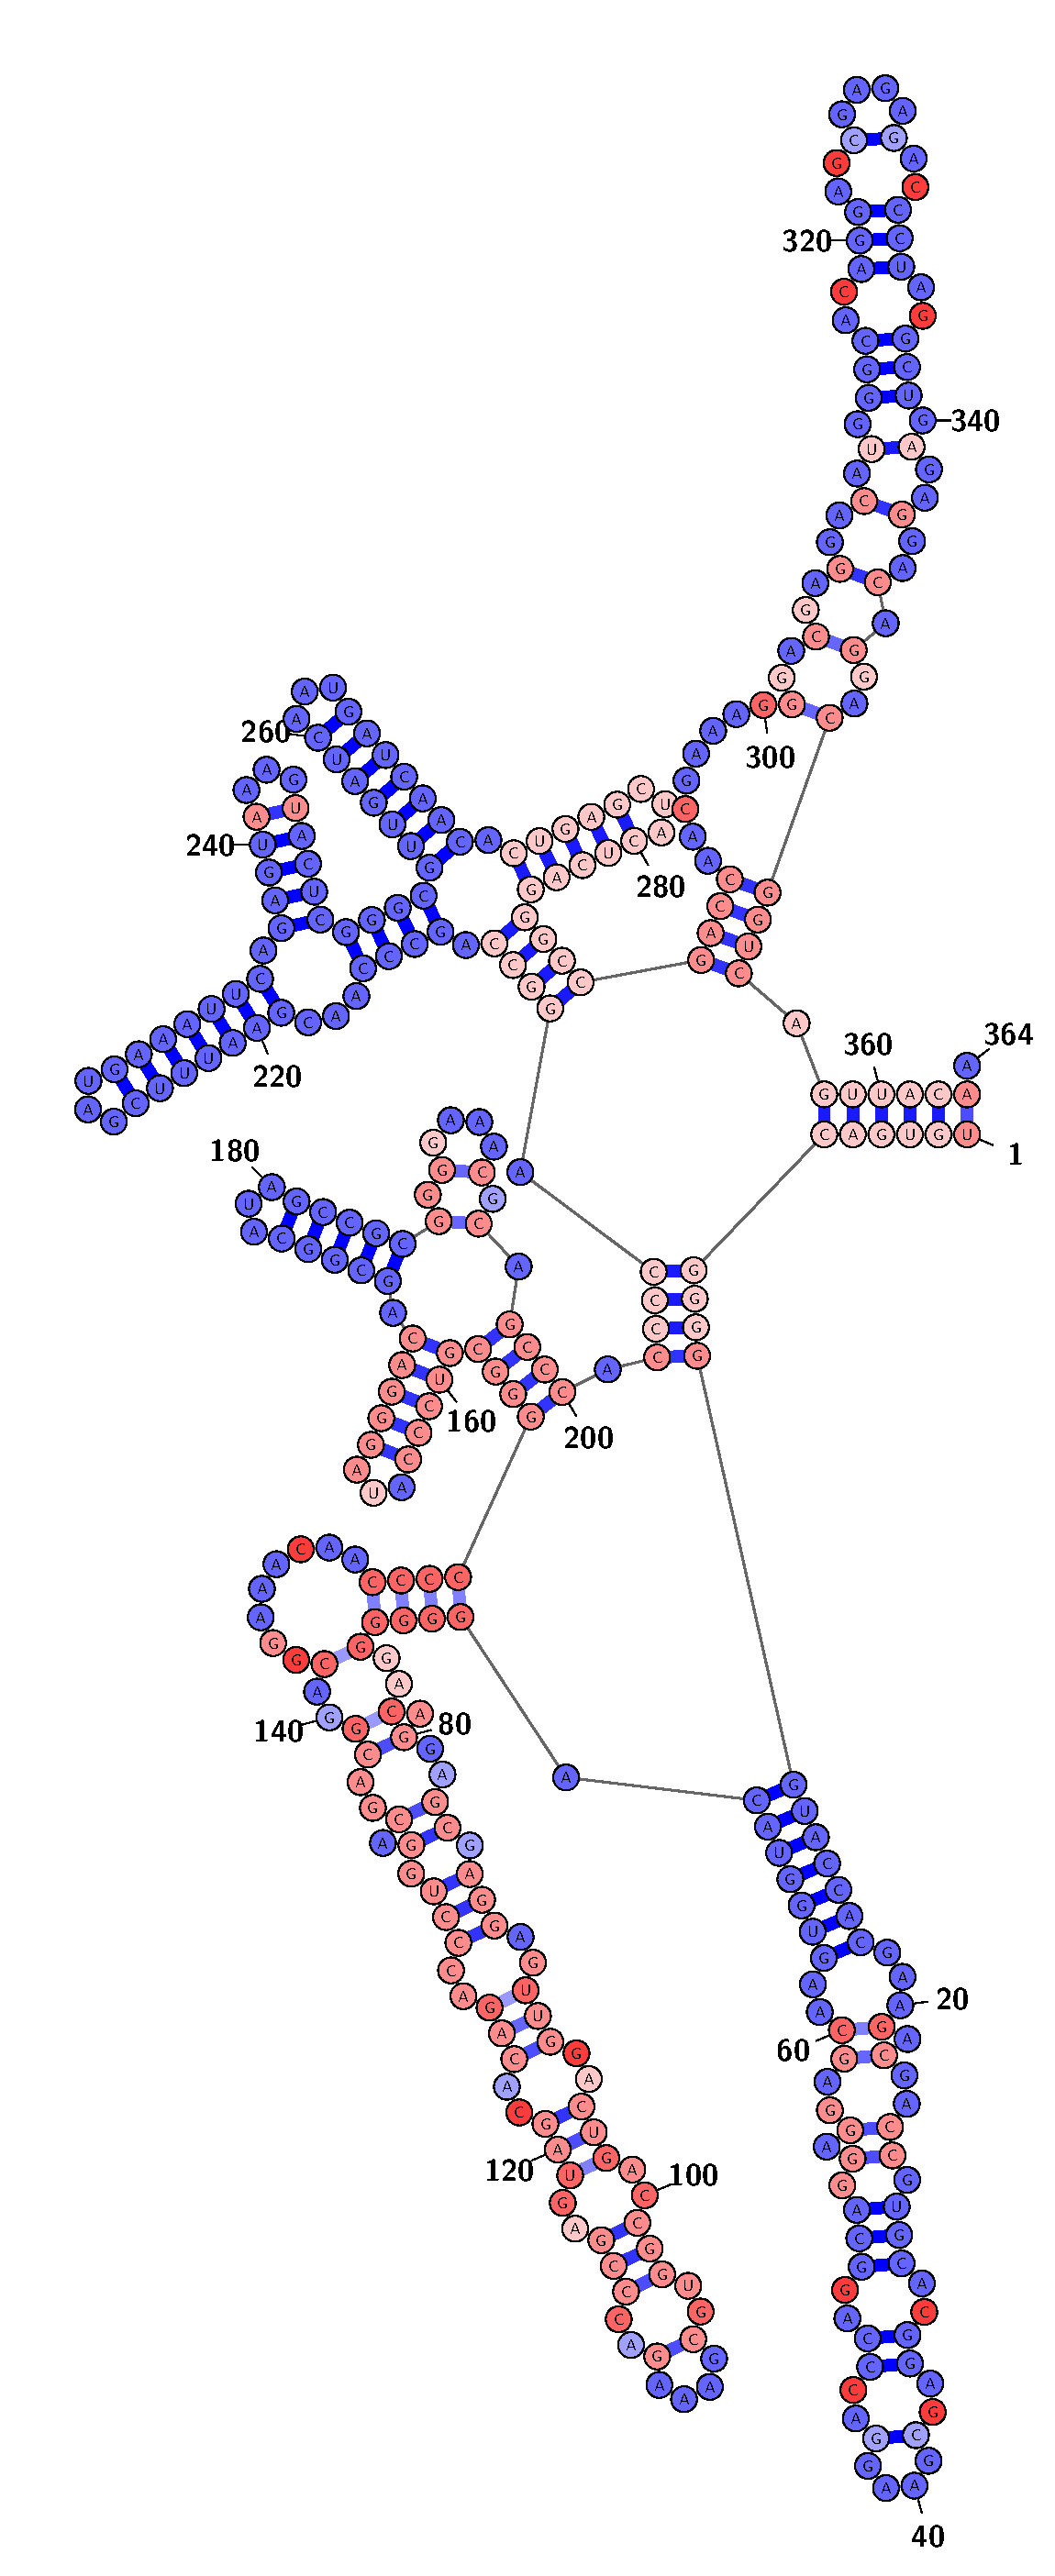
\includegraphics[height=4.85in]{figures/structures/structure_99_sampling}
\end{tabular}\\[3pt]
\begin{tabular}{@{}c@{\hspace{0.02\linewidth}}c@{}}
(e) Base-pairing probabilities, EliteDesign ($N=500$) & (f) Base-pairing probabilities, SamplingDesign \\[1pt]
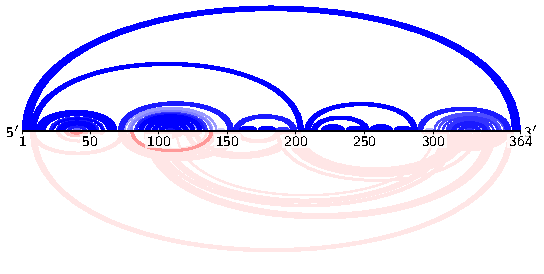
\includegraphics[width=0.49\linewidth]{figures/structures/arcs_99_elite} &
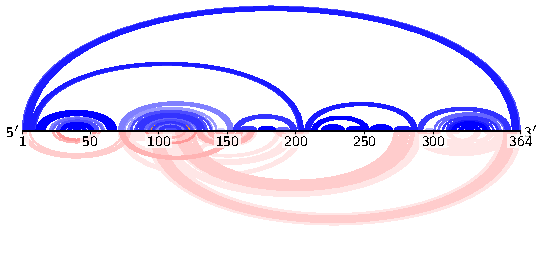
\includegraphics[width=0.49\linewidth]{figures/structures/arcs_99_sampling}
\end{tabular}}
\caption{This figure shows the sequences with the highest Boltzmann probability from EliteDesign ($N=500$) and SamplingDesign on Puzzle \texttt{\#99} (``Shooting Star''), which is a proven undesignable puzzle. (a) The scores of each design and a probability upper bound on $p(\vecystar\mid\vecx)$~\citep{zhou2026}. (b) The target structure \vecystar. (c)--(d) The MFE structure of each design. Nucleotides are colored by positional defect. For these MFE predictions, all pairs also belong to \vecystar, and the shade of blue indicates the probability, with darker being higher. (e)--(f) Base-pairing probabilities, where blue arcs are the pairs that match between a structure $\vecy'$ in the ensemble and \vecystar, orange arcs are matching pairs with a probability under 0.1, and red arcs are the pairs of $\vecy'$ that do not match \vecystar. Darker arcs have higher probability.}
\label{fig:eterna-structure-99}
\end{figure}
